\begin{activity} \label{A:5.2.1}  Suppose that $f$ is the function given in Figure~\ref{F:5.2.Act1} and that $f$ is a piecewise function whose parts are either portions of lines or portions of circles, as pictured.
\begin{figure}[h]
\begin{center}
\scalebox{0.85}{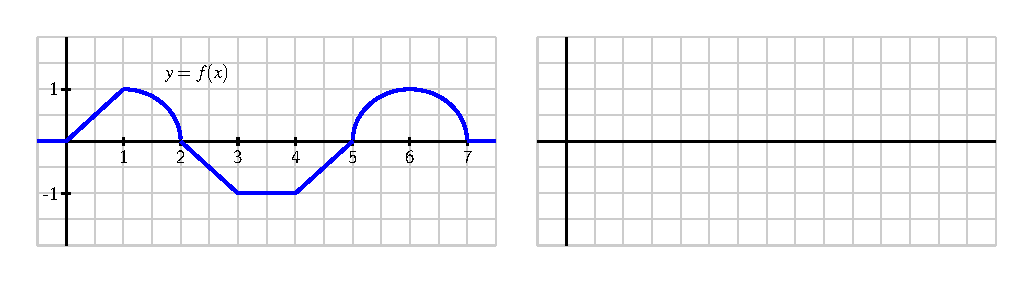
\includegraphics{figures/5_2_Act1.eps}}
\end{center}
\caption{At left, the graph of $y = f(x)$.  At right, axes for sketching $y = A(x)$.} \label{F:5.2.Act1}
\end{figure}
In addition, let $A$ be the function defined by the rule $A(x) = \int_2^x f(t) \, dt$.
\ba
	\item What does the Second FTC tell us about the relationship between $A$ and $f$?
	\item Compute $A(1)$ and $A(3)$ exactly.
	\item Sketch a precise graph of $y = A(x)$ on the axes at right that accurately reflects where $A$ is increasing and decreasing, where $A$ is concave up and concave down, and the exact values of $A$ at $x = 0, 1, \ldots, 7$.
	\item How is $A$ similar to, but different from, the function $F$ that you found in Activity~\ref{A:5.1.1}?
	\item With as little additional work as possible, sketch precise graphs of the functions $B(x) = \int_3^x f(t) \, dt$ and $C(x) = \int_1^x f(t) \, dt$.  Justify your results with at least one sentence of explanation.
\ea
\end{activity}
\begin{smallhint}
\ba
	\item If you don't recall it, review the statement of the Second FTC above.
	\item Note that $A(1)= \int_2^1 f(t) \, dt$.
	\item Don't miss our key conclusion from (a).
	\item Compare the values of $A(1)$ and $F(1)$.
	\item What does the Second FTC tell us about the relationship between $B$ and $f$?
\ea
\end{smallhint}
\begin{bighint}
\ba
	\item Review the statement of the Second FTC above; what does that theorem tell you about $A'$?
	\item Note that $A(1)= \int_2^1 f(t) \, dt$; don't forget that $\int_2^1 f(t) \, dt = -\int_1^2 f(t) \, dt$.
	\item Don't miss our key conclusion from (a), which enables us to gain information from the derivative of $A$ about where $A$ is increasing, decreasing, concave up, and concave down.
	\item Compare the values of $A(1)$ and $F(1)$; note that $F$ could be equivalently defined by the rule $F(x) = \int_0^x f(t) \, dt - 1$.
	\item What does the Second FTC tell us about the relationship between $B$ and $f$?  Between $C$ and $f$?  Note, too, that we can write $B(x) = F(x) - F(3)$, where $F$ is any antiderivative of $f$.
\ea
\end{bighint}
\begin{activitySolution}
\ba
	\item By the Second FTC, $A'(x) = f(x)$.
	\item Since $A(1)= \int_2^1 f(t) \, dt = -\int_1^2 f(t) \, dt$, it follows $A(1) = -\frac{\pi}{4}$.
	\item Note that $A$ is increasing wherever $f$ is positive, and $A$ is CCU wherever $f$ is increasing.  Similar conclusions follow for $A$ being decreasing and/or concave down.  Moreover, $A(2) = 0$, $A(3) = -0.5$, $A(4) = -1.5$, $A(5) = -2$, $A(6) = -2 + \frac{\pi}{4}$, and $A(7) = -2 + \frac{\pi}{2}$.
	\item In our current example, $A$ is an antiderivative of $f$ that satisfies $A(0) = -\frac{1}{2} - \frac{\pi}{4}$.  Our earlier work with $F$ showed that $F$ is an antiderivative of $F$ that satisfied $F(0) = -1$.  Since $F$ and $A$ are both antiderivatives of $f$, they differ by a constant, and that constant is $-1 - (-\frac{1}{2} - \frac{\pi}{4}) = \frac{\pi}{4} - \frac{1}{2}$.
	\item The Second FTC tells us that $B' = f$ and $C' = f$.  Thus, $B$ and $C$ are each antiderivatives of $f$, have the same shape as $A$ and $F$, and each differ from $A$ by just a constant.  Observing that $B(3) = 0$ and $C(1) = 0$ enables us to easily sketch these shifted versions of $A$.
\ea
\end{activitySolution}
\aftera